\documentclass[class=article]{standalone}

%\documentclass[12pt,a4paper]{article}
%
%\usepackage{../preambolo}
%
%\usepackage[
%style=numeric,
%natbib=true,
%backend=biber,
%sorting=ynt,
%maxbibnames=99
%]{biblatex}
%\addbibresource{../bibliografia.bib}

\begin{document}
%\justifying
\section{Indicatori}
	Numerosi sono gli studi condotti al fine di comprendere lo stile di guida adottato dal conducente di un veicolo, tuttavia la maggior parte di questi si sono focalizzati sulle automobili.
	In questi articoli la componente \(z\) dell'accelerazione e le rotazioni attorno agli angoli di \(rollio\) e \(beccheggio\) sono stati trascurati in quanto ritenuti poco rilevanti per descrivere il comportamento dinamico dalle automobili.
	Una bicicletta, però, si muove in modo significativamente differente rispetto a un'auto.
	In particolare, durante le curve, la bicicletta ruota sia attorno all'asse di \(rollio\) che a quello di \(beccheggio\) mentre lungo l'asse \(z\) è possibile osservare la forza centrifuga.
	
	
	Negli articoli consultati, gli indicatori più comunemente utilizzati sono risultati essere media, varianza e distanza picco-picco. Oltre a quelli citati, però, ne sono stati utilizzati degli altri. In particolare, l'articolo \cite{chen}, riguardante lo stile di guida delle automobili, fornisce una lista molto completa di indicatori e sperimenta l'introduzione di nuovi come, per esempio, lo shape factor e il margin factor.\hfill\break
	
	
	Durante questa ricerca sono stati utilizzati i seguenti indicatori:
	\begin{itemize}
		\item Indicatori temporali
		\begin{itemize}
			\item Media (\(mean\)), Valor Medio Rettificato (\(arv\)) e Media Quadratica (\(rms\))
			\item Varianza (\(var\)) e Deviazione Standard (\(std\))
			\item Kurtosis (\(krt\))
			\item Skewness (\(skw\))
			\item Massimo (\(max\)), Minimo (\(min\)) e Distanza Picco-Picco (\(pk\))
		\end{itemize}
		\item Indicatori adimensionali
		\begin{itemize}
			\item Shape factor (\(sf\))
			\item Crest factor (\(cf\))
			\item Impulse factor (\(if\))
			\item Margin factor (\(mf\))
		\end{itemize}
		\item Indicatori basati sulla frequenza
		\begin{itemize}
			\item Ampiezza media (\(amp\))
			\item Frequency centroid (\(cnt\))
			\item Varianza delle frequenze(\(fvar\))
			\item Entropia spettrale (\(ent\))
		\end{itemize}
	\end{itemize}
	
%	magari aggiungere la tabella con le formule
	
	Questi indicatori sono stati applicati ai dati provenienti dall'accelerometro, dal giroscopio e dal magnetometro e alla velocità durante le fasi di accelerazione, curva e frenata. Di seguito verranno descritti gli indicatori che si sono rivelati più interessanti durante le tre fasi appena citate.
	
	\begin{center}
		\begin{figure}[h]
			\centering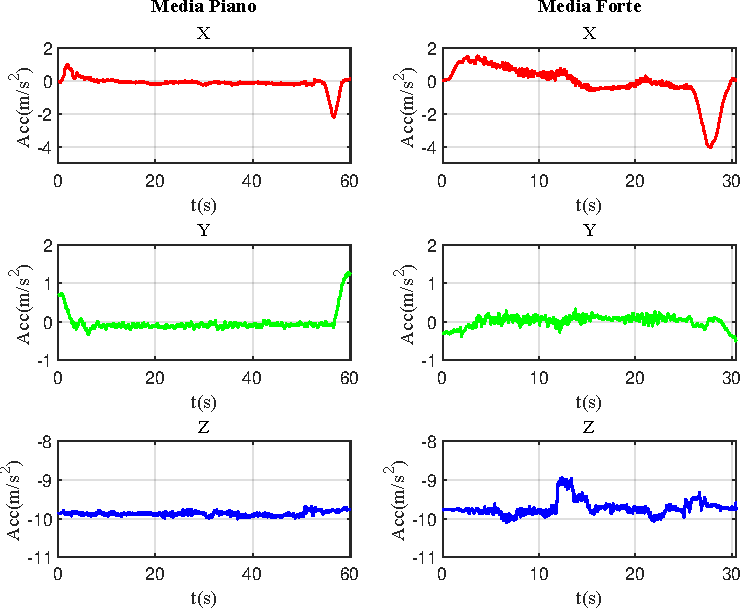
\includegraphics[width=.9\textwidth]{img/lungaFP/Acc/Media}
			\caption[]{}
			\label{fig:AccMedia_lungaFP}
		\end{figure}
	\end{center}
	
	\begin{center}
		\begin{figure}[h]
			\centering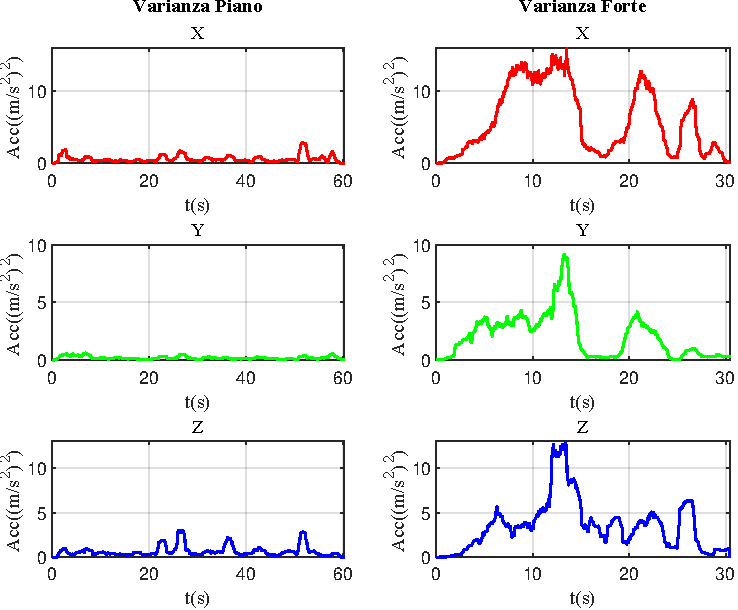
\includegraphics[width=.9\textwidth]{img/lungaFP/Acc/Varianza}
			\caption[]{}
			\label{fig:AccVar_lungaFP}
		\end{figure}
	\end{center}
	
	\begin{center}
		\begin{figure}[h]
			\centering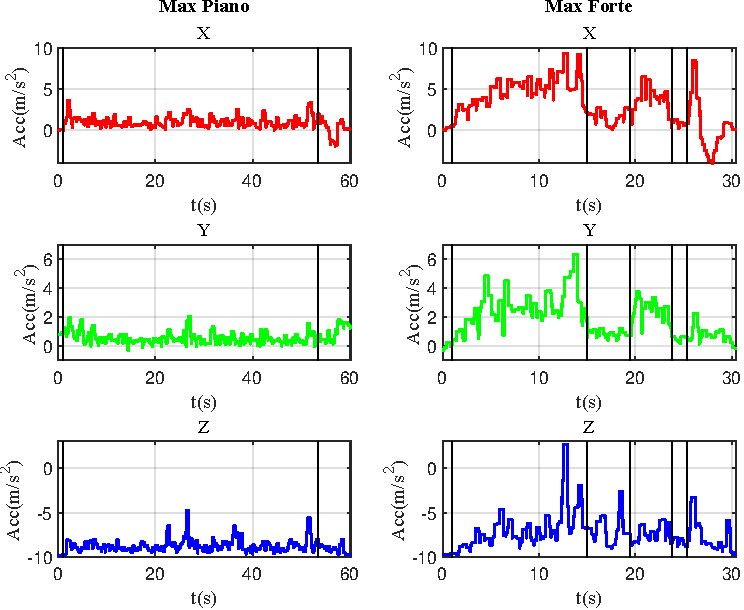
\includegraphics[width=.9\textwidth]{img/lungaFP/Acc/Max}
			\caption[]{}
			\label{fig:AccMax_lungaFP}
		\end{figure}
	\end{center}
	
	\begin{center}
		\begin{figure}[h]
			\centering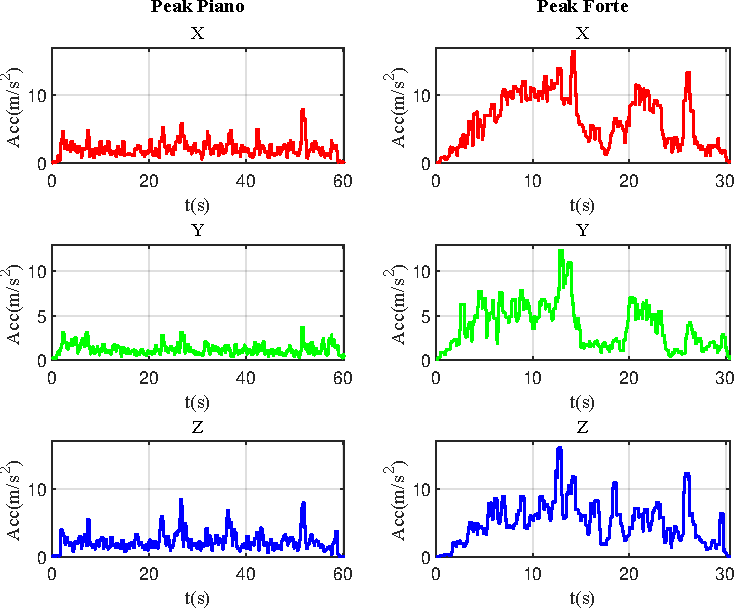
\includegraphics[width=.9\textwidth]{img/lungaFP/Acc/Peak}
			\caption[]{}
			\label{fig:AccPeak_lungaFP}
		\end{figure}
	\end{center}
		
	\subsection{Accelerazione e Frenata}
	Durante le fasi di accelerazione e frenata gli indicatori che si sono rivelati maggiormente utili sono:
	\begin{itemize}
		\item media accelerazione in \(x\)
		\item varianza accelerazione in \(x\) e \(y\)
		\item massimo accelerazione in \(x\)
		\item distanza picco-picco accelerazione in \(x\) e \(y\)
		\item varianza velocità in \(x\)
		\item distanza picco-picco velocità in \(x\)
		\item deviazione standard \(rollio\)
		\item distanza picco-picco \(rollio\)
	\end{itemize}
	
	\begin{center}
		\begin{figure}[h]
			\centering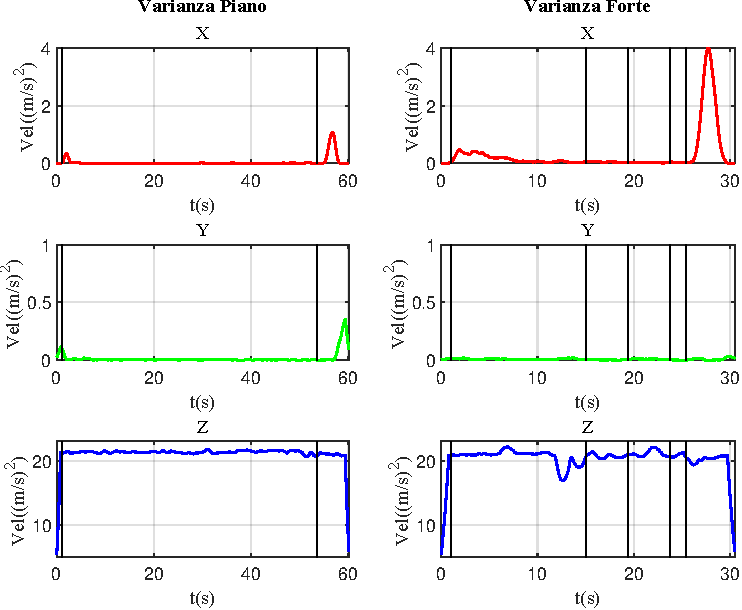
\includegraphics[width=.9\textwidth]{img/lungaFP/Vel/Varianza}
			\caption[]{}
			\label{fig:VelVar_lungaFP}
		\end{figure}
	\end{center}
	
	\begin{center}
		\begin{figure}[h]
			\centering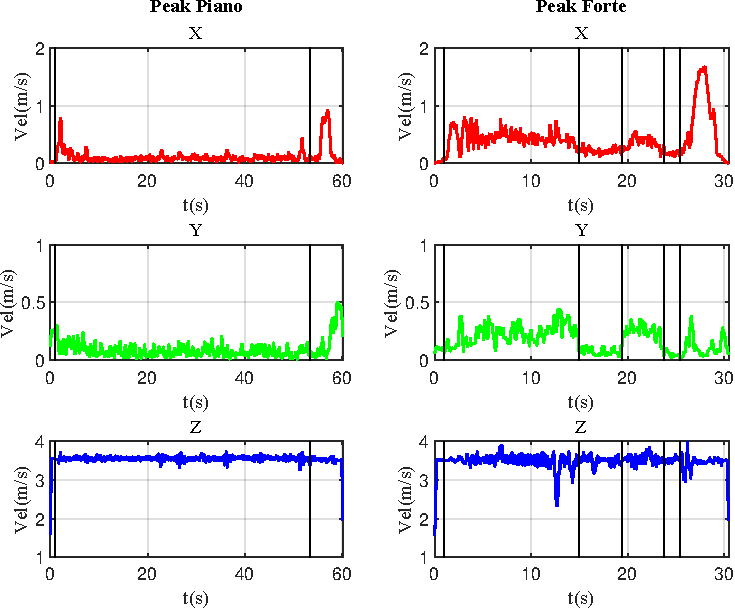
\includegraphics[width=.9\textwidth]{img/lungaFP/Vel/Peak}
			\caption[]{}
			\label{fig:VelPeak_lungaFP}
		\end{figure}
	\end{center}
	
	\begin{center}
		\begin{figure}[h]
			\centering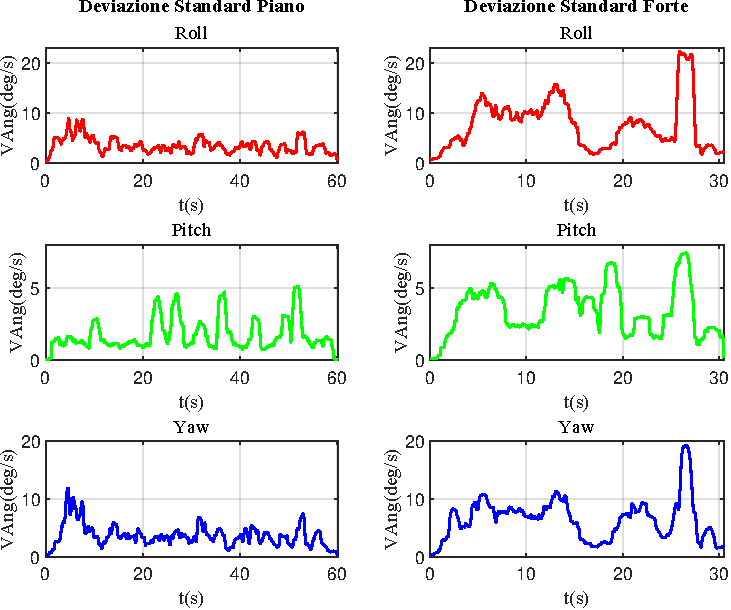
\includegraphics[width=.9\textwidth]{img/lungaFP/VAng/Deviazione Standard}
			\caption[]{}
			\label{fig:VAngStd_lungaFP}
		\end{figure}
	\end{center}
	
	\begin{center}
		\begin{figure}[h]
			\centering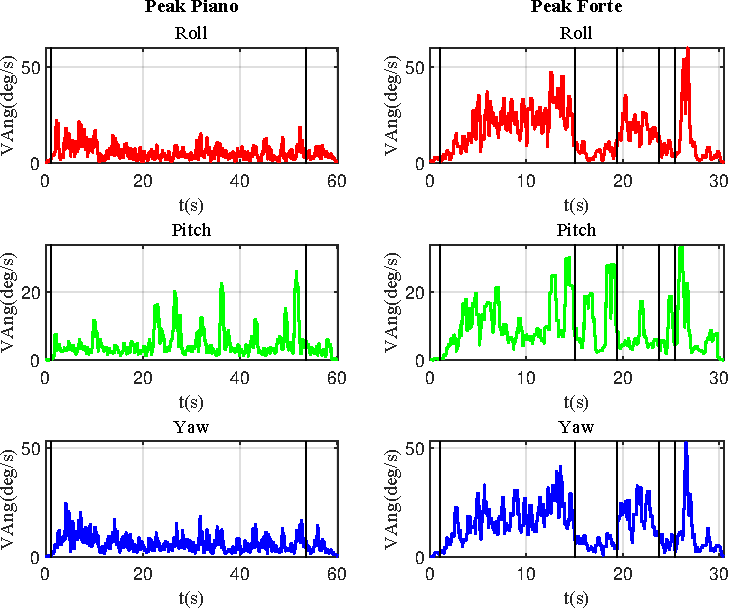
\includegraphics[width=.9\textwidth]{img/lungaFP/VAng/Peak}
			\caption[]{}
			\label{fig:VAngPeak_lungaFP}
		\end{figure}
	\end{center}
	
	L'andamento medio dell'accelerazione in \(x\), calcolata come media degli ultimi \(1.6s\), mostra un incremento durante le fasi di accelerazione della bicicletta che tende a diminuire fino a \(0\) all'aumentare della velocità.
	Risulta essere negativa solo nei momenti in cui il ciclista smette di pedalare, procedendo per inerzia, e quando frena. In quest'ultimo caso è visibile una netta e rapida diminuzione di questo parametro in funzione dell'intensità della frenata.
	
	Per quanto riguarda la media rettificata, la media quadratica, la varianza e la deviazione standard dell'accelerazione lungo gli assi \(x\) e \(y\) hanno tutte un andamento molto simile. Di questi parametri è stata selezionata la varianza in quanto ha un range di valori più ampio e consente, quindi, una migliore identificazione degli eventi. In particolare la varianza lungo gli assi \(x\) e \(y\) è in grado di evidenziare lo sforzo del ciclista nel pedalare, con valori tanto più elevati quanto più l'accelerazione lungo questi assi oscilla. La varianza dell'accelerazione in \(x\) è inoltre in grado di evidenziare le frenate.
	Anche il massimo dell'accelerazione in \(x\) si comporta come la varianza, con la differenza che le frenate vengono segnalate con un valore negativo più o meno evidente a seconda del numero di dati utilizzati per calcolarlo. Questo rende più facile distinguere le fasi di accelerazione dalle fasi di frenata.
	
	Comportamento analogo a quello della varianza è stato osservato nella distanza picco-picco dell'accelerazione degli assi \(x\) e \(y\).\hfill\break
	
	Per quanto riguarda la velocità, sia la varianza che la deviazione standard identificano molto bene le frenate.\hfill\break
	
	Come per l'accelerazione anche nel caso della velocità angolare dell'angolo di rollio la media rettificata, la media quadratica, la varianza e la deviazione standard hanno comportamenti simili che identificano bene la foga con cui il ciclista pedala, così come la distanza picco-picco del rollio.\hfill\break
	
	Il campo magnetico, infine, non fornisce molte informazioni per quanto riguarda i percorsi rettilinei.
	
	\subsection{Curva}
	Durante la fase di curva gli indicatori che si sono rivelati maggiormente utili sono:
	\begin{itemize}
		\item media accelerazione in \(x\)
		\item varianza accelerazione in \(x\)
		\item varianza velocità in \(x\)
		\item distanza picco-picco velocità in \(x\)
		\item media \(beccheggio\) e \(imbardata\)
		\item deviazione standard \(rollio\) e \(imbardata\)
		\item massimo \(beccheggio\) e \(imbardata\)
		\item media campo magnetico in \(x\)
		\item varianza campo magnetico in \(x\)

	\end{itemize}
	
%	L'accelerazione media lungo l'asse \(x\) è in grado di rilevare le curve in quanto, durante queste, si nota una decelerazione della bicicletta.
	
	L'accelerazione media lungo l'asse \(x\) mostra una decelerazione durante le curve, rendendo così possibile una loro identificazione.
	
	Anche in questo caso media rettificata, media quadratica, varianza e deviazione standard dell'accelerazione lungo \(x\) hanno un andamento molto simile e mostrano un picco durante le fasi di curva.\hfill\break
	
	Per quanto riguarda la velocità, gli indicatori varianza e deviazione standard rilevano le curve in corrispondenza del rallentamento della bicicletta durante le stesse.\hfill\break
	
	La velocità angolare è un ottimo modo per riconoscere le curve. La media della velocità angolare degli angoli di \(rollio\), \(beccheggio\) e \(imbardata\) riesce a fornire una chiara indicazione di quando avviene una curva. Tra questi, si distinguono in particolare gli ultimi due. La media del \(beccheggio\) fornisce informazioni sull'entità della curva e sulla velocità alla quale la si sta percorrendo: più ampia è la curva minore sarà il suo valore, maggiore è la velocità della bicicletta più questo sarà elevato. Il \(beccheggio\) non può, però, fornirci informazioni sul verso della curva stessa. Per risalire a questa informazione è stata selezionata l'\(imbardata\). Anche il massimo di questi angoli si comporta in modo analogo.
	
	Infine, nella varianza e nella deviazione standard degli angoli di \(rollio\) e \(imbardata\) è possibile notare due picchi all'inizio e alla fine della curva.\hfill\break
	
	La varianza del campo magnetico in \(x\) mostra dei picchi, più o meno pronunciati, a seconda dell'orientamento della bicicletta all'inizio e alla fine della curva.
	
	\subsection{Utilizzo degli Indicatori}
	Lo studio fatto serve per selezionare un'insieme di indicatori che consentano di dedurre l'impegno che il ciclista mette nel pedalare o in grado di identificare uno specifico evento come curve e frenate.
	
	Dalla varianza dell'accelerazione dell'asse \(x\) è possibile rilevare in modo efficace l'oscillazione della stessa, dovuta alla foga che il ciclista mette nel pedalare. Maggiore è la varianza, tanto più il ciclista sta pedalando velocemente. Di conseguenza, quando il ciclista procede per inerzia senza pedalare, la varianza risulta essere molto bassa.
	
	Grazie alla media dell'accelerazione in \(x\) si può, invece, dedurre l'efficacia della pedalata: più la media è elevata, maggiore è l'accelerazione della bicicletta e, quindi, maggiore è l'utilità dello sforzo del ciclista.
	
	L'accoppiata varianza e media dell'accelerazione in \(x\) sono quindi in grado di determinare lo sforzo impiegato nel pedalare e la sua efficacia.
	
	Dalla sola varianza non è però possibile distinguere la foga del ciclista dalle curve e dalle frenate. In queste occasioni, infatti, la varianza si comporta nello stesso modo.
	
	Questo problema si può risolvere utilizzando la varianza dell'accelerazione lungo l'asse \(y\), che, pur con meno precisione, registra principalmente l'impegno del ciclista escludendo curva e frenate.
	
	Un'altra possibilità è controllare quando la media dell'accelerazione diventa negativa. Questo succede solamente in quei momenti in cui la bicicletta rallenta, ovvero quando procede per inerzia e, sopratutto, quando curva o frena.	
	
	In alternativa, accoppiando la varianza dell'accelerazione dell'asse \(x\) con altri indicatori, in grado di rilevare specificatamente curve e frenate, è possibile discernere se il valore è riferibile alla foga o meno.
%	Questi indicatori sono: la varianza della velocità in \(x\) per le frenate e la media della velocità angolare del \(beccheggio\) e dell'\(imbardata\) per capire quando sta curvando.
	
	Analogo discorso si può fare con gli indicatori distanza picco-picco e media rettificata che hanno un andamento simile a quello della varianza.\hfill\break
	
	Per quanto riguarda il rilevamento delle curve e della loro intensità abbiamo la media o il massimo della velocità angolare di \(beccheggio\) e \(imbardata\). In particolare il primo si dimostra molto efficace a identificare la velocità alla quale viene percorsa in quanto, in base a quest'ultima, cambia l'inclinazione della bicicletta e, quindi, la velocità di rotazione attorno all'angolo di \(beccheggio\). Grazie all'\(imbardata\), invece, possiamo capire il verso di rotazione della bicicletta.
	
	La varianza del campo magnetico lungo l'asse \(x\), infine, riesce a identificare la differenza tra l'orientamento iniziale e finale della curva.\hfill\break
	
	La frenata, invece, si rileva in modo efficace grazie varianza della velocità in \(x\), che mostra un picco tanto più evidente quanto maggiore è la differenza di velocità della bicicletta prima e dopo la frenata. Per questo motivo è in grado di evidenziare anche curve e i momenti di forte aumento di velocità, in particolare quando la bicicletta parte da ferma, seppur in modo molto meno marcato.
	
	Discorso analogo può essere fatto con la distanza picco-picco e con la deviazione standard, in questo caso, però, è meno evidente la differenza tra frenate e curve.
		
\end{document}